\section{Alert Production in Commissioning and Early Operations}
\label{sec:pp}

\subsection{Processing Overview}

The \DPDD{} summarizes the pipelines which will be used during Prompt Processing to produce alerts as well as other prompt data products, including Solar System Processing.
In brief, raw images have instrument signatures removed and are photometrically and astrometrically calibrated.
When template images for the corresponding region of the sky are available, the template is subtracted from the new processed visit image and sources are detected on the image difference.
Alerts are then generated for all DIASources detected at five sigma in the difference.
At the end of the night, DIASources without a history of previous detection are input into Solar System Processing, which attempts to link them with other past detections and identify new Solar System objects.

Both Alert Production and Solar System Processing thus depend on the presence of template images.
During steady-state operations, these templates will be constructed during the annual Data Releases and will be built from the best available subset of images taken.
The input images for DRP-produced templates will accordingly have very good seeing and comprehensive spatial coverage.
All of these template characteristics help to ensure that image differencing is highly complete and highly pure.

To enable alert production to proceed during commissioning and early operations, it is necessary to accept templates of lower quality.
Because we have a smaller set of input images to choose from and uncertain knowledge about future observations, on-the-fly (or incremental) template generation necessarily must balance the trade off of earlier template availability against template quality and spatial completeness.
Substantial validation will be required to determine when to build incremental templates to maximize the net throughput of Early Science.
Nevertheless our goal is to enable Alert Generation to begin over at least a subset of the survey area as soon as the data are scientifically useful.

Coadding multiple images enables artifact rejection  \citeds{DMTN-080} and is formally required due to the noise-level requirements placed on the DM system. 
Additionally, the LSST survey is heavily dithered, so without coadding many images onto a common sky plane it is both difficult and inefficient to obtain image differences for a new pointing from past single images.
Finally, single-image templates do not permit removal of artifacts, transients, and moving objects from the template, creating additional false positive sources in the resulting differences.

Scientifically it is important that once a template is constructed for a given region of sky, it is used exclusively until it can be updated in the next Data Release.
Repeated changes to the template make it extremely difficult to construct usable lightcurves for objects from individual difference image sources: transient objects such as supernovae will be contaminated by changing flux levels from the evolving template, and variable objects such as variable stars and AGN will require repeated corrections for different template flux levels as well.

\subsection{Supporting Incremental Template Generation}

The Rubin Construction Data Management (DM) Science team (DM-SST) carried out a study of several options for Alert Production in Year 1, reported in \citeds{DMTN-107} : Options for Alert Production in LSST Operations Year 1.
Representatives of the Rubin Project Science Team (PST), DM-SST and Operations reviewed the proposed DM-SST options  and converged on a the following  strategy for Alerts in year 1:

\begin{itemize}
\item Commissioning Data Templates: Build templates, where possible, from all commissioning data before the start of year one, and use them to generate alerts during year one.
\item Year One Data Templates: Build templates progressively from data obtained during year one (e.g., on a monthly timescale), and use them to generate alerts during year one, either instead of, or in addition to using commissioning data to build templates.
\end{itemize}

To handle alert generation outside the template building process attached to the annual DRP, the Construction project initiated a change request to include incremental templates in the DM system workflow. This change has been accepted and is now part of the baselined DM project in construction. A summary of the changes is the following:

\begin{itemize}
\item LCR-2273: Construct Image Differencing Templates Outside DRP, new requirement 1.4.6 Template Coadds ID: DMS-REQ-0280, The DMS shall periodically create Template Images in each of the u,g,r,i,z,y passbands. Templates may be constructed as part of executing the Data Release Production payload, or by a separate execution of the Template Generation payload. Prior to their availability from Data Releases these coadds shall be created incrementally when sufficient data passing relevant quality criteria is available.
\item To enable artifact rejection, templates will be built with at least three images in year one, and five in subsequent years (Rubin OSS-REQ-0158). \footnote{The LSST SRD places well-defined criteria on the quality of the difference image and the amount of noise that a template can contribute to a difference image.These criteria result in a minimum of three images being needed to construct a template for use in year one, and five in subsequent years.}
\item Once a template is produced for a sky position and filter it will not be replaced until the next Data Release to avoid repeated baseline changes.
\item Templates are not necessarily built from the first N images that are collected.
\end{itemize}


\subsection{Alert Generation during Commissioning}

Due to the need to verify the instrument characteristics, template quality, and image differencing and Real/Bogus performance, real-time alerts will not be immediately available during the commissioning period.
However, the incremental template generation and alert production processes will be tested and optimized during commissioning with LSSTCam, resulting in a set of prompt data products, including alerts.
Broker teams will be given access to these alerts for development purposes as soon as they are produced to understand their characteristics and to help to validate their quality, rather than to enable rapid followup and Early Science.
The Alert and Prompt Product databases will be made available for query prior to the DP2 data release.

During commissioning templates will be generated incrementally over the maximal sky area supported by the available observations.
By the end of the commissioning period, coadd templates for use in difference imaging will only be available for $\approx$ 10\% of the sky.
Generating templates over a wide area is not an explicit goal of commissioning;  however, where possible, if commissioning observations are agnostic to pointing and filter, we would endeavour to choose a pointing and filter that maximizes building templates to enable early science.

Rubin aims to scale up alert production during commissioning with the aim of beginning routine Alert Production as soon as is feasible following System First light.
Once begun, Alert Production will then proceed continuously into the full LSST survey.
Alerts generated during commissioning may be produced with higher latency.
The commissioning period also provides an excellent opportunity to investigate how many visits in a given band are sufficient to construct a usable template.

The prompt data products, including Alerts, generated during commissioning and the first year of the LSST survey are summarized in Table~\ref{tab:prompt-products}.

\begin{table}[ht]
\centering
\label{tab:prompt-products}
\caption{Summary of prompt data products expected during commissioning and year 1 survey observations, as of January 2023.}
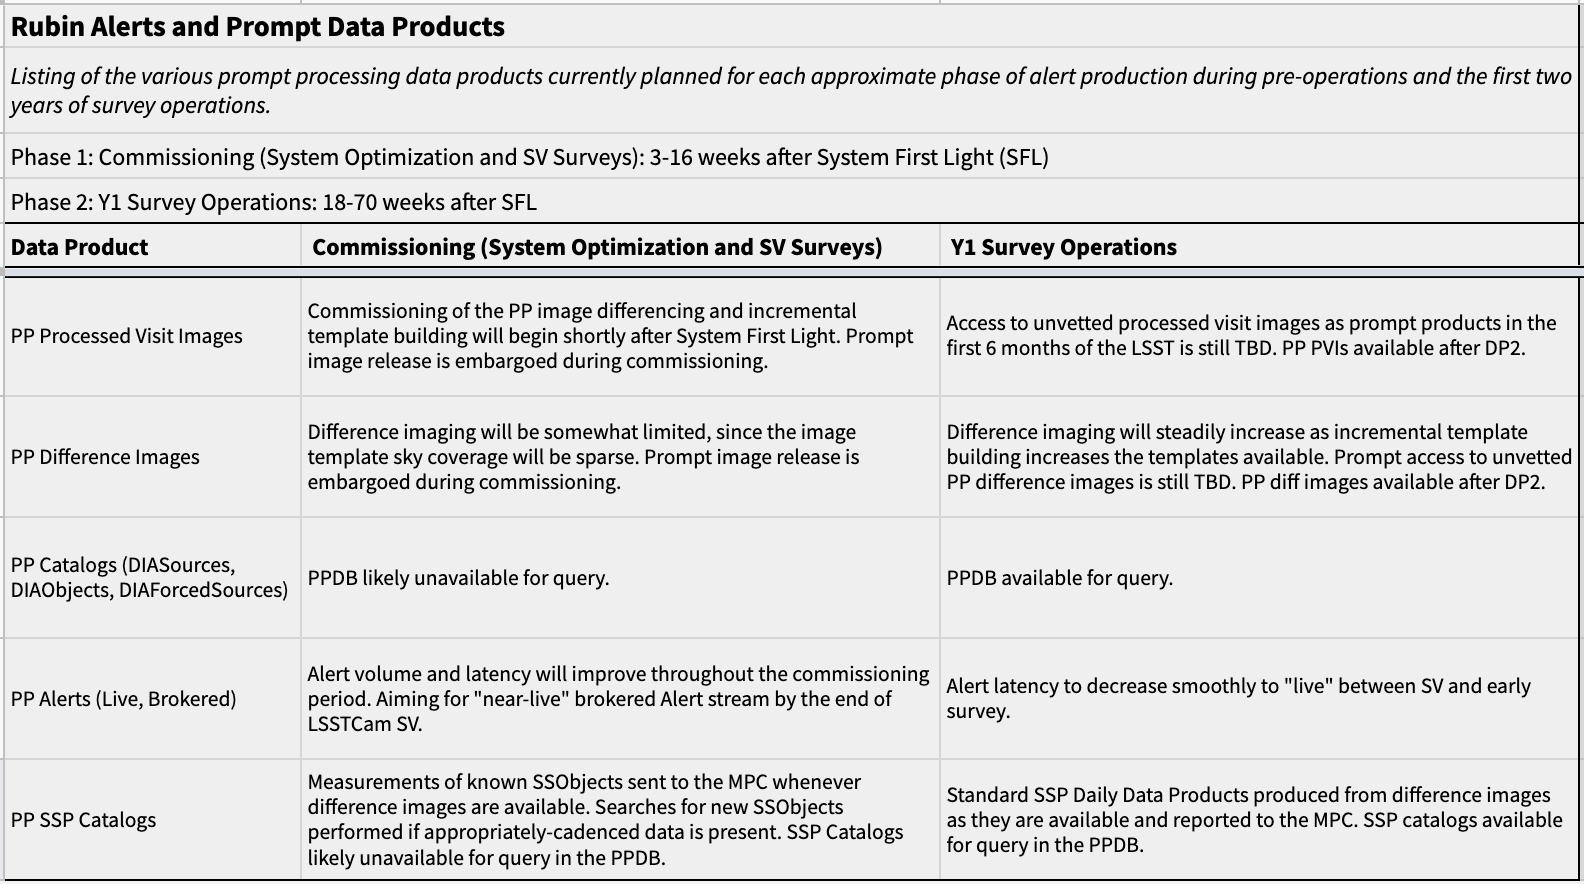
\includegraphics[width=0.9\linewidth]{figures/Prompt-products}
\end{table}
